\chapter{General Introduction}

\section{The ocean, phytoplankton and why it matters}
The complexity of the ocean and its vast ecosystems has fascinated scientists to this day and most likely will continue to do so far into the future. Myriad life forms are embedded in a matrix so far removed from our mostly dry existence on top the earth’s crust. In the ocean, life moves in dilution, and the equivalents of forests and grasslands are hard to spot unless the concentration of tiny phytoplankton is so large, that deep blue turns into a milky green.

The term phytoplankton refers to microscopic marine photosynthetic organisms. These microorganisms form the basis of the oceanic food web and are primary producers of planetary scale, contributing roughly half of the oxygen in our atmosphere through photosynthesis \citep{Field2009}. Phytoplankton consists of mostly single-celled organisms, prokaryotes and eukaryotes from a highly diverse evolutionary background \citep{Falkowski2004a}. This large genetic diversity is accompanied by a remarkable range of survival strategies, biogeochemical roles, shapes and sizes within the polyphyletic phytoplankton (see Figure \ref{FinkelPhySizeRange} for a size comparison). 
The emergence of such a large range of organisms and the mechanisms sustaining their persistence has been one of the key topics in phytoplankton ecology over the last 50 years. Hutchinson's paradox.X(REF here)X

\begin{figure}
\centering
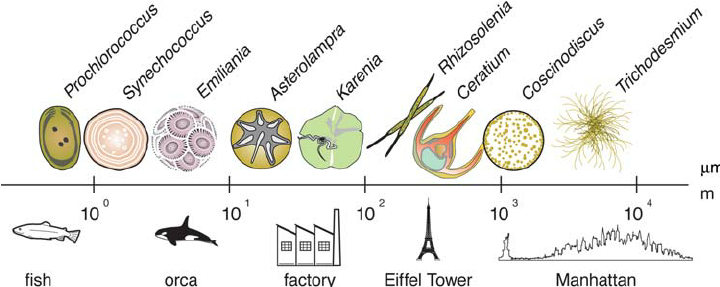
\includegraphics[trim = 0mm 0mm 0mm 0mm, clip, width=.9\linewidth]{./Chp1-Intro/SIZEphytoComparison_FinkelEtAl2010.png}
\caption[Scheme]{\small {"A comparison of the size range (maximum linear dimension) of phytoplankton
relative to macroscopic objects." from \cite{Finkel2010}}}
\label{FinkelPhySizeRange}
\end{figure}

||| also explain MLD in the following paragraph |||

The distribution of phytoplankton is driven by the complex physical forces that govern ocean currents and the chemistry of the bodies of water the move. The key components are macronutrients (e.g. nitrogen \& phosphorus) and micronutrients (e.g. iron \& cobalt) welling up from the deeper ocean or flushed in from continental sources. Wherever there are sufficient nutrients available within the euphotic zone, the depth where photosyntheticaly available radiation (PAR) is 1\% of the surface value, planktonic life begins to thrive. Ecosystems along continental margins provide a particularly productive habitat, with only 10\% of total ocean surface area covered by continental margins, but 10-15\% of marine primary production and more than 40\% of carbon export to the seabed occurring along coastal lines \citep{Yool2001,Muller-Karger2005}.


Phytoplankton growth indirectly feeds a considerable part of earth’s population through fisheries \citep{Stock2017} and even shapes the elemental composition of oceanic water itself \citep{Redfield1958}. 
The biomass produced is mostly consumed by higher trophic levels and either assimilated or excreted. Another large portion experiences natural mortality and viral lysis. Microbial degradation drives remineralization within the euphotic zone, which fuels regenerated production \citep{Eppley1979} [Perhaps put quotation about Microbial Loop here!]. 
A small fraction sinks out of the photic layer as fecal or detrital matter to the deeper ocean and an even smaller fraction reaches the sea floor as sediment ( roughly 1 \%) and remains there over geological times \citep{Honjo2008}. This process has been termed the biological carbon pump. Carbon sequestered this way is removed from the ocean-atmosphere system for potentially millions of years. Given the projected rise of atmospheric CO$_2$ levels, it is of grave importance to understand how changes in the phytoplankton community at the surface, driven by anthropogenic stressors and climate change, will affect the carbon burial potential of oceanic ecosystems. 
Studies have both reported a global declining trend in marine primary production \citep{Boyce2012} and increasing trends in long-term ocean time series \citep{Chavez2011a}. 
In order to answer questions of how phytoplankton will respond to a changing climate it is necessary to look the diverse phytoplankton community in greater detail. 

\section{Characterizing phytoplankton communities}
From the early days of oceanographic research, scientists have been interested in the microscopic organisms that were floating in samples of sea water. These communities contain many species each and in total there are tens of thousands of species of phytoplankton that inhabit the surface ocean \citep{DeVargas2015}. All phytoplankton species use chlorophyll or bacteriochlorophyll to harvest light as the energy source to fix organic carbon, but there is wide variation in virtually all their other properties \citep{Litchman2008}. In addition to the complex community composition, there are many factors affecting measurements of their bulk properties in the ocean, such as the viral and bacterial community and the influence of diverse grazers, all within the complex three-dimensional physical environment that is the ocean. 
Where earlier phytoplankton ecologists focused on identifying individual species, decoding their phylogeny or growing them in controlled lab cultures, recent research is trying to integrate the insights gained from these approaches and quantify the diversity on higher levels of organization in relation to other properties of the ecosystem. The focus has shifted towards trait diversity both within and across species and within and across phytoplankton groups. In order to scientifically describe this perplexing diversity the concepts of trait-based ecology and functional types have been developed \citep{Tilman2001,McGill2006,Violle2007c}.

\begin{figure}
\centering
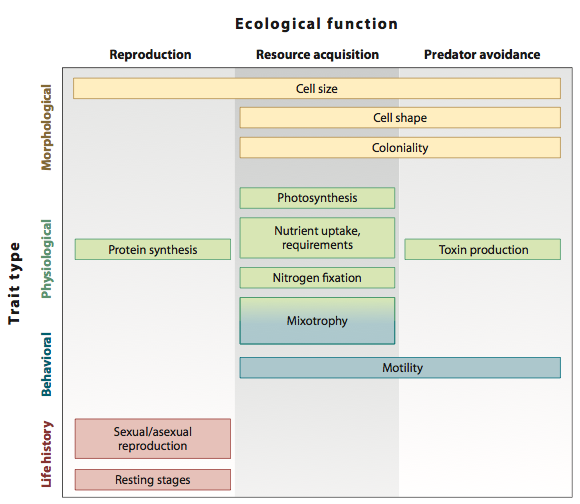
\includegraphics[width=0.7\linewidth]{./Chp1-Intro/Fig_litchman2008.png}
\caption[Scheme]{\small{"A typology of phytoplankton functional traits" from \cite{Litchman2008}}}
\label{PhytoTraits}
\end{figure}

\small {\textbf{Functional types, traits and diversity}}

In the following I will try to clarify the complementary terms of phytoplankton traits, functional traits, and functional types. 

The trait-based approach to phytoplankton ecology has been growing in popularity. Part of the fascination evoked by this term stems from its origin in evolutionarily theory. Over the last three decades, it has been adopted by ecologists trying to understand communities and ecosystems. In this new context, the concept of traits has been stretched far beyond its original meaning, which can lead to some confusion surrounding the scope of trait-based methods \citep{Violle2007c}. In the simplest definition, a trait is a surrogate of organismal performance. In the ecological context this has been expanded to surrogates for the performance of populations, communities and entire ecosystems. This can include ecophysiological traits, life-history traits, demographic traits or response and effect traits of ecosystems (see Figure \ref{PhytoTraits} for a selection of phytoplankton traits). Theoretically, any property of an organism or ecosystem could be defined as a trait, but ideally a trait should be functional. Functional traits are defined by \cite{Violle2007c} as "morpho-, physio- or phenological traits which impact fitness indirectly via their effects on growth, reproduction and survival". An important facet of the trait-based approach is to describe organismal function via trade-offs between traits. For example when competing for multiple nutrients, phytoplankton species are thought to be constrained by trade-offs in their competitive ability for one over another resource \citep{Tilman1990}. 

Phytoplankton are extremely diverse and the trait based approach lends itself to generalizations, as traits and ecological trade-offs can be defined and explored irrespective of species or taxa boundaries \citep{McGill2006}. However, depending on the study and hypotheses to be tested, it can be very helpful to structure the diversity of organisms into distinct groups. Major taxonomic groups of phytoplankton can be classified based on their ecological or biogeochemical roles within the ecosystem \citep{Iglesias-Rodriguez2002,Flynn2015}. The concept of functional groups is not in contrast to a trait-based ecology of phytoplankton, but can be complementary to it. By broadly sampling relevant traits across phytoplankton groups and species, functional types can be defined by functional traits and trade-offs and therefore extend the trait-based approach by another level of organization \citep{Litchman2007d}. An early example is the work of Ramón Margalef. Margalef used observations of important traits, such as sinking rates and nutrient utilization to build the concept called "Margalef's mandala" to organize phytoplankton functional types (PFTs) on a spectrum of nutrient availability versus turbulence \citep{Margalef1978}. 

The terms functional group and functional type are used interchangeably, with functional groups more often referring to the grouping of species and the functional type describing the group as a whole, often as implemented in computational models. In fact, the simplification of the phytoplankton community into functional types has been widely used for the design and interpretation of computational models that try to recreate or make predictions about the biogeochemical cycling, biogeographic distribution, productivity and other ecosystem functions of phytoplankton \citep{Gregg2003,LeQuere2005}. Biogeochemically defined functional types are most often used, as these functional traits can usually be well defined within an ecosystem model. Typical examples of such functional groups are silicifers, which broadly correspond the phylogenetic group of diatoms, and calcifiers, which are usually represented by coccolithophores. Such functional types are always simplifications of the natural pyhtoplankton diversity. Silicoflagellates create silicified skeletons like diatoms, but are often not explicitly included because they rarely dominate modern phytoplankton assemblages. The choice of which functional groups to include in a model can also be driven by biogeography or analytical considerations concerning the measurement instrumentation used for a particular study \citep{IrwinAndrewJ.Finkel2017b}. 

||||Perhaps small paragraph about functional diversity here?||||
In biodiversity research, the trait-based approach has been readily adopted. It used to be that species diversity (i.e. the number of species) was the most important metric, but now it is functional diversity, which can be described by the variance in the value of a functional trait of the community or ecosystem.

It is important to keep in mind that functional types are often composed of many species with a possibly large variance in trait values. Recent research is trying to understand the effects of diversity within functional types and within species \citep{Violle2012,Violle2017a,DesRoches2018}.




\section{Modeling phytoplankton communities}
Given the complexity of the ocean ecosystem, it is necessary to aggregate our knowledge of the many smaller parts into comprehensive ecological models in order to test mechanistic hypotheses and investigate their full-scale implications. 

Computational models of phytoplankton growth have been developed since the 1940s and have greatly increased in sophistication and complexity since then, co-evolving with the rise in computational resources \citep{Gentleman2002a}. Phytoplankton modelling started with formulations based on the Lotka-Volterra equations of predator-prey dynamics \citep{Fleming1939}. From these relatively simple descriptions models evolved to describe the oceanic physical environment and the ecosystem it contains including multiple trophic levels. Originally developed by John Steele with a model ocean split in two layers, the nutrient-phytoplankton-zooplankton (NPZ) and nutrient-phytoplankton-zooplankton-detritus (NPZD) models succeeded in reproducing the typical annual bloom dynamics observed in the temperate ocean \citep{Steele1958,Evans1988,Fasham1990a}. Further developments have been in more exact physiological descriptions of phytoplankton based in cellular metabolism and energy allocation \citep{Geider1997} and both simple and more complicated ecosystem formulations driven by local and global 3D circulation models \citep{Lacroix2007, Hirata2013}.

However, in their simplified approach, these models unavoidably limit the characterization of a diverse phytoplankton community \citep{Bruggeman2009}. These plankton ecosystem models are typically highly aggregated, such that a single variable determines the response of a diverse assemblage of phytoplankton species \citep{Franks2009}. Implementing a meaningful treatment of biodiversity in ecological models is a key challenge in the field of phytoplankton modeling \citep{Queiros2015}. The most apparent way of implementing this within the framework of established NPZD models is to include multiple equations and state variables for different phytoplankton functional types \citep{LeQuere2005}. For every group that fulfills a distinct ecosystem function, a new set of parameters has to be added, which complicates the model structure and increases computational costs. This somewhat intuitive approach, however, does lead to problems. First and foremost, this is the lack and inherent uncertainty of data from field and culture experiments to constrain functional types. This again leads to the difficulty of validating the model output in light of insufficient information, leading multiple authors to criticize the PFT modeling approach as attempting to "run before we can walk" particularly when used for extrapolating into the future \citep{Anderson2005,Shimoda2016}. 

The current scientific discussion can seem intimidating to an early career scientist, as both the most obvious future directions of ecosystem model design as exemplified by PFT models, as well as the very foundation of traditional NPZD models has come under scrutiny. Nowhere is this more apparent as with the formulation of nutrient uptake dynamics, which is traditionally defined by Monod kinetics that are based on the equations for Michealis-Menten enzyme kinetics. (Monod reference here)

ALSO: current modeling paradigms are discussed quite critically in the literature, in particular the Monod kinetics and also the lack of any adaptive mechanisms in these model \citep{Smith2014}
A bit earlier, but similar direction: \citep{Flynn2010}
and more recent, but focused on Monod: \citep{Hellweger2017a}

However, there are also examples of modeling approaches that show a way forward. To name an alternative to the modeling paradigm discussed so far, there is individual based modeling (IBM). In IBM the phytoplankton are explicitly represented as individual agents, allowing for a diverse and spatially interactive phytoplankton community \citep{Hellweger2009}. The computational cost and structural complexity of this approach however does not yet lend itself well to studies of large-scale or even global ecosystems. 

Another approach which lends itself very well to just such studies is to extend traditional NPZD models via moment-based estimation of aggregate properties \citep{Merico2009}. A specific implementation of this is the PhytoSFDM model developed by \citet{Acevedo-Trejos2016}. Instead of modeling multiple size-classes of phytoplankton explicitly, the community is described not only by the biomass, but also by the mean size and size variance. Size is used as a master trait, with size variance being used as a proxy for functional diversity. Trade-offs related to nutrient uptake, grazing and sinking structure the phytoplankton community along the size spectrum as driven by the physical forcing. The model was used to investigate latitudinal diversity gradients in the Atlantic Ocean \citep{Acevedo-Trejos2018}. One point of criticism for this approach is that due to the mathematical structure the size distribution is fixed to the shape of a skewed log-normal distribution, not allowing for the emergence of other (e.g. multi-modal) distributions that could arise in natural phytoplankton communities (Urusla Gercke, Tony Klaus, Francesco paper on size dist in lakes). This lends the PhytoSFDM model (in it's current formulation) more to studies of large scale processes and biogeographic patterns rather than to local ecosystem modeling studies.

looking at aggregate properties, how complex model has to be, how simple it has to be, aggregate model can not capture all of the variability, model capturing all of variability (Hellweger, Science article, biogeographic patterns emerging - GLOBAL FIX ERROR BEFORE)

1. very complex -> IBM
2. DARWIN
3. aggregate with adaptive dynamics and PhytoSFDM, similarly to optimality based model
I am for interemdiate levels of optimality
Tom Anderson "Running before we can walk"

ALSO: problem of looking at within FT diversity, look at the details of diversity -> including PFTs very complicated!

perhaps not cutting edge, but my method allows me to catpure variability wihtin functional groups!

don't rubbish other models/papers

A major advancement in the field of phytoplankton modeling was the DARWIN model developed at MIT \citep{Follows2007d}. In the general framework of the DARWIN model, large numbers of phytoplankton types are initialized with equal biomass but with different parameters for the most important traits, namely those related to light harvesting, temperature dependence, and nutrient acquisition. These parameters are chosen stochastically from broad ranges of values, based on laboratory and field data, and constrained by simplified allometric functions describing ecological trade-offs. Different functional types are prescribed in the model via varying nutrient utilization traits (e.g. small phytoplankton that cannot assimilate nitrate as Prochlorococcus analogs). Over multi-annual runs this community self-assembles through ecological competition and physical changes produced by the simulated environment of a global circulation model (GCM). In the random initialization of phytoplankton types, the DARWIN model allows for the emergence and development of diverse phytoplankton communities. This approach of modeling biodiversity has been termed “selection-based” \citep{Follows2011c}. ||more attention to this review|| The model framework is continually modified and expanded, for example for exploring the effect of grazing formulations \citep{Prowe2012c}, the biogeography of phytoplankton traits \citep{Barton2013} and the influence of ocean acidification at a global scale \citep{Dutkiewicz2015}. 
Size structured ecosystem models have been done before: \citep{Baird2007b}
A study of particular interest is the size-structured food-web model component developed by \citet{Ward2012}, because the modeling approach combines the trait-based approach of scaling parameters allometrically along cell size with a PFT modeling approach. Each functional type is assigned a different allometry based on the size ranges and relationships taken from data. Together with the selection-based biodiversity representation that the DARWIN framework provides, this seems to be a promising direction for future models. The model has however only been applied and compared to data at a global scale and the code of this specific implementation is not publicly available.

PhytoFLEX -> Systems of infinite Diversity ->
structure paragraph along axis of complexity?

ALWAYS NEED A GOOD BASIS IN DATA TO VALIDATE MODELS AND HYPOTHESES

\section{The Cariaco Basin and the CARIACO time-series}
\label{CARIACOintro}

At the beginning of my PhD I was tasked with the mission to find publicly available ocean time-series data that could be used as the basis for my modeling work. Initially the plan was to choose multiple locations, to compare results from model applications in contrasting environments. Not surprisingly the search did quickly yield results, among the most prominent: the Bermuda Atlantic Time-series Study (BATS) and the Hawaii Ocean Time-Series (HOTS). Quickly the issues of public ocean time-series data became apparent. Links often lead to defunct sites and servers were sporadically maintained. In particular for my application the problem was that the basic physical parameters and bulk properties such as total chlorophyll were readily available, but more specific phytoplankton functional type or taxonomy data was harder to find, if not missing. In particular the type of phytoplankton data that was available differed widely between the stations and would have not allowed for a straightforward comparison. It was only later in my search that I came across the CARIACO time series, an acronym for "CArbon Retention In A Colored Ocean", located in the Cariaco Basin off the coast of Venezuela. The data is available through the University of South Florida (USF) at \href{http://imars.marine.usf.edu/cariaco}{http://imars.marine.usf.edu/cariaco} and includes a wealth of data that was collected since 1995. Most importantly to my purposes, the data included both phytoplankton pigment measurements and taxonomic data of the phytoplankton community at monthly intervals. It was the first ocean time-series with such detailed public phytoplankton data and soon I decided to focus my work on this time-series.

In addition to the recent importance of the cariaco basin as the site of an important paleo-oceanographic time sereis, the Cariaco basin has served as a natureal laboratory for biogeochemists for over 50 years. This basin has been key in constructiong stoichiometric models of organic matter remineralization (Redfield et al 1963 and Richards 1975!), developing residence time and box models, and numerous other studies.

Cariaco basin is the worlds largest truly marine anoxic basin \citep{Wakeham2012}.


|||perhaps what is above is not entirely needed --> maybe less colloquial, more why CARIACO is interesting! ||||||

THE BASIN
The CARIACO Ocean Time-Series program was established in 1995 off the coast of Venezuela (10$^\circ$ 30$'$ N, 64$^\circ$ 40$'$ W, see Figure \ref{CARIACO-map}). Located in the south-eastern Caribbean Sea, the Cariaco Basin is a 160 km long and 70 km wide tectonic depression, reaching up to 1400 m in depth. The two deeper parts of the basin are separated by a saddle of 900 m depth, with the time-series mooring located in the eastern part. The entire basin is bound to the west and north by a shallow ridge at 100 m depth, restricting the exchange of deep water with the Caribbean Sea. The restricted circulation and high productivity at the surface resulted in anoxic conditions below 250 m depth within the basin \citep{Richards1956}. The hydrography at the surface is influenced by Guyana and North Equatorial currents that flow into the Caribbean Sea from a south-eastern direction, but this exchange is restricted to the two channels above the 100 m ridge. Observed and modeled horizontal surface water velocities within the basin are relatively weak, indicating a minimal influence of horizontal transport at the mooring site \citep{Alvera-Azcarate2009}. 

\begin{figure}
\centering
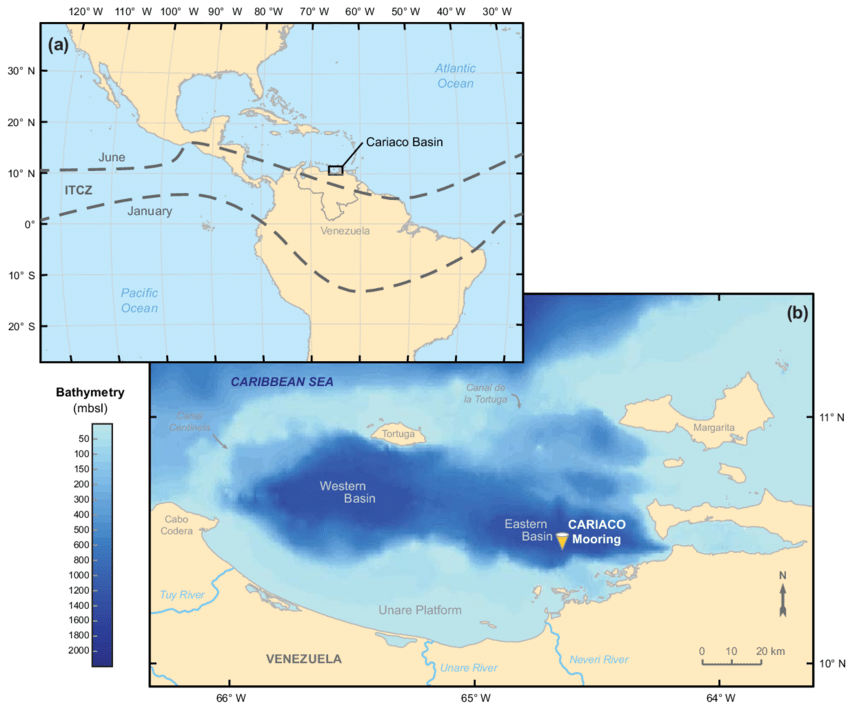
\includegraphics[trim = 0mm 0mm 0mm 0mm, clip, width=1.\linewidth]{./Chp1-Intro/CARIACObasinMAP_Bringueetal2018.png}
\caption[Scheme]{\small {"Study area. A. Location of the Cariaco Basin off the Venezuelan coast in the southern Caribbean Sea, with January and June positions of the Intertropical Convergence Zone (ITCZ). B. Location of the CARIACO station in the eastern sub-basin, general bathymetry and local rivers emptying in the basin (bathymetric data from GEBCO\_08 Grid)" from \cite{Bringue2019}}}
\label{CARIACO-map}
\end{figure}


SAMPLE COLLECTION
The program was established as a joint-project of the Venezuelan Fondo Nacional de Cienca, Tecnolog\'{i}a e Investigac\'{i}on (FONACIT) and the US National Science Foundation (NSF), with the particular interest in creating a time-series of surface ocean biogeochemistry that could be linked to satellite observations and the sedimentation accumulating in the anoxic basin. Since 1995 there were over 200 core cruises at mostly monthly intervals, in addition to sediment trap and microbial-biogeochemistry process cruises. 


MEASURED DYNAMICS
Simply mention the major publications and rough findings, further discussion in section 2

perhaps here:
inter-annual and subdecadal variability in nutrient geochemistry \citep{Scranton2014}


LONG TERM TRENDS <- not here, but discuss this in the 2nd section (MS 1)

SCIENTIFIC FINDINGS - RESULTS what has been found here?

- Interesting: Novel eukaryotes found at Oxic-Anoxic interface \citep{Stoeck2003}

Say that JPinckney loves me
and how this is a promising data set, given the history, wealth of data, incl phytoplankton diversity data, and long term trends here.

ALSO: Time series has stopped, due to lack of funding, and cite review paper (scientific legacy of CARIACO) \citep{Muller-Karger2019a}
Perhaps here go through the main points in the big review to give a nice overview


% keep muthsinda et al and all that jazz to the next section, lessgo

XXXXXXXXXXXXXXXXXXXXXXXXXXXXXXXXXXXXXXXXXXXXXXXXXXXXXXXXXXXXXXXXXXXXXX

%Primary productivity in the basin is high (over 300 g C m−2 yr−1) and shows great seasonal and interannual variability (e.g., Müller- Karger et al., 2001, 2004). Seasonal upwelling of Subtropical Under- water (SUW: salinity of 36.9, nitrate concentration of 5–10 μM; Morrison and Smith, 1990) is controlled by the position of the Inter- tropical Convergence Zone (ITCZ). Between December and April, the ITCZ typically lies south of the equator and strong E–NE trade winds (> 6m s−1) induce upwelling along the coastline, fostering high levels of primary productivity (e.g., Richards, 1975; Müller-Karger et al., 2001). During the summer/fall rainy season, the ITCZ migrates to its northern position, winds weaken and upwelling ceases, although shorter, secondary upwelling events are often observed, particularly in July and August (e.g., Astor et al., 2003; Goñi et al., 2003). Pronounced interannual variations in primary productivity were also observed at the CARIACO station (located in the eastern sub-basin), with annually- integrated measurements between 1996 and 2001 ranging from ∼370 to 650 g Cm−2 yr−1 (Müller-Karger et al., 2004). Surface salinity at the CARIACO station typically varies only slightly, from>36.8 in Ja- nuary–July to<36.6 during the rainy season (Astor et al., 2003). The dominant modes of climatic variability known to influence the
%region include the North Atlantic Oscillation (NAO) and the El Niño–Southern Oscillation (ENSO) phenomenon. Phases of the NAO, defined as the difference in sea level pressure anomalies between the Azores High and the Icelandic Low, are known to modulate precipita- tion in the Caribbean (e.g., Giannini et al., 2001) but appear to have limited impact on the hydrography and SST patterns of the basin (e.g., Taylor et al., 2012; Astor et al., 2013). ENSO affects a major portion of the tropical Pacific, the Americas and the Caribbean through atmo- spheric teleconnections, and it has been shown to influence precipita- tion, SST and productivity patterns at the CARIACO station with a one year lag (Enfield and Mayer, 1997; Giannini et al., 2001; Taylor et al., 2012; Astor et al., 2013). ENSO may also cause shifts in phytoplankton communities in the basin (Goñi et al., 2003; Romero et al., 2009; Bringué et al., 2018). The high levels of primary production result in the export of large
%fluxes of particulate organic matter to the depths (Thunell et al., 2000, 2007),2007), while the Tuy, Unare, and Neveri rivers (Fig. 1) deliver the bulk of terrigenous sediments to the basin (e.g., Elmore et al., 2009; Bout- Roumazeilles et al., 2013). The succession of intervals of high primary productivity in surface waters during active upwelling (and associated flux of biogenous material), and periods of low productivity and rainy conditions when sedimentation is dominated by lithogenous particles, is reflected in the basin’s laminated sediments that accumulate under anoxic conditions (e.g., Peterson et al., 1991; Hughen et al., 1996; Thunell et al., 2000; Goñi et al., 2003).

SAMPLE COLLECTION
%This study uses samples collected as part of the Cariaco Ocean Time-Series Program at a station located in the eastern basin (10°30′ N, 64°40′ W; Fig. 1). The CARIACO station has been the site of oceano- graphic observations since 1995, with monthly water column sampling and nearly continuous deployment of sediment traps (Thunell et al., 2000; Müller-Karger et al., 2001). Monthly water column sampling included Conductivity-Temperature-Depth (CTD) casts, providing tem- perature, salinity and σT profiles, and sampling at discrete depths using a rosette equipped with 12 Teflon-coated Niskin bottles, for measure- ments of various parameters including dissolved oxygen, pH, alkalinity, Chlorophyll a concentrations (Chl a), phaeopigments and nutrients, rates of primary productivity, suspended particulate organic carbon and nitrogen. An overview of the program and methods is provided in Müller-Karger et al. (2001), and sampling, analytical procedures and data are available at www.imars.usf.edu/cariaco. Since

SEA SURFACE DYNAMICS
%Contour plots showing the evolution of temperature, σT, PO4 and Chl a over the duration of the time series are presented in Fig. 2. The most striking feature in these records is the seasonal upwelling cycle that brings colder (see Temperature panel; Fig. 2A), nutrient-rich wa- ters (exemplified by PO4 and Si(OH)4; Fig. 2C and D) to the surface and promotes primary productivity (Chl a; Fig. 2E), typically observed during winter and spring of each year, but with additional, shorter ‘secondary’ upwelling events often recorded later in summer months (e.g., Jul.–Aug. 1997, Jul. 1998, Jul. 2002, Jul.–Aug. 2003, Jul. 2004, Jul.–Aug. 2006). The other major observation is that there is con- siderable interannual variability in terms of upwelling strength and duration, with some years showing particularly strong and/or sustained upwelling (in particular, 1997, 2000, 2001, 2003, 2006, 2007 and 2008) while others are marked by much weaker and/or shorter active upwelling intervals (e.g., 1999, 2004, 2005). In order to better char- acterise the variability in upwelling state and associated biological re- sponse, the practical classification of active (weak, moderate and strong) and relaxed upwelling conditions proposed by Bringué et al. (2018) and supported by previous observations in the basin (e.g., Müller-Karger et al., 2001; Astor et al., 2003; Goñi et al., 2003; Taylor et al., 2012; Rueda-Roa et al., 2018) was used. Such intervals are de- fined on the basis of isotherms reaching a depth of 50 m, determined from temperature measurements at the study site (Fig. 2A). Conditions of ‘weak’, ‘moderate’ and ‘strong’ upwelling correspond to intervals when the 22, 21 and 20 °C isotherms reach 50m depth, respectively, and are indicated in Figs. 3–6 and 8–42 by blue3, shaded areas. All other intervals (when temperatures at 50m are>22 °C) are considered to represent ‘non-active’ upwelling conditions, with ‘neutral’ conditions defined as intervals when the 23 °C isotherm reaches a depth of 50 m, and all other (warmer) intervals corresponding to ‘relaxed’ upwelling conditions. Over the duration of the time series, temperature in the upper 100m of the water column varied between 19 and 30 °C, with the lowest temperatures typically observed at depth and during active upwelling intervals, and the highest values recorded at the surface during up- welling relaxation (Fig. 2A). 


LONG TERM TRENDS 

%-> Go For TAYLOR et al 2012! And mention updated Phyto ChlA dynamics from Pinckney, leave all the rest to section 2

 

XXXX

XXXX

XXX

THEN TALK ABOUT THE COLLABorDATASHARE WITH JPINCKNEY AND CBENITEZNELSON, and how this allows an even deeper look at the biomass dynamics


\section{Aims of the proposed PhD project}
"The general goal of my Ph.D. project is to study the processes that structure the phytoplankton community in contrasting environmental regions of the Atlantic Ocean, using a trait-based modelling perspective. The specific aims during the course of the project are to:

\begin{itemize}
\item MANUSCRIPT 1 "Understanding Shifts in CARIACO"
\item MANUSCRIPT 2 "technical paper" - Geoscientific Model development
\item MANUSCRIPT 3 "BDEF in CARIACO"
\end{itemize}
